\addcontentsline{toc}{chapter}{Appendix C: Schematics}  
\chapter*{Appendix C: Schematics}
\label{chap:appendix-C-schematics}

\section*{Buck converter schematic} \label{Appendix_buck_schematic}
\addcontentsline{toc}{section}{Buck converter schematic}
\begin{figure}[ht]  
    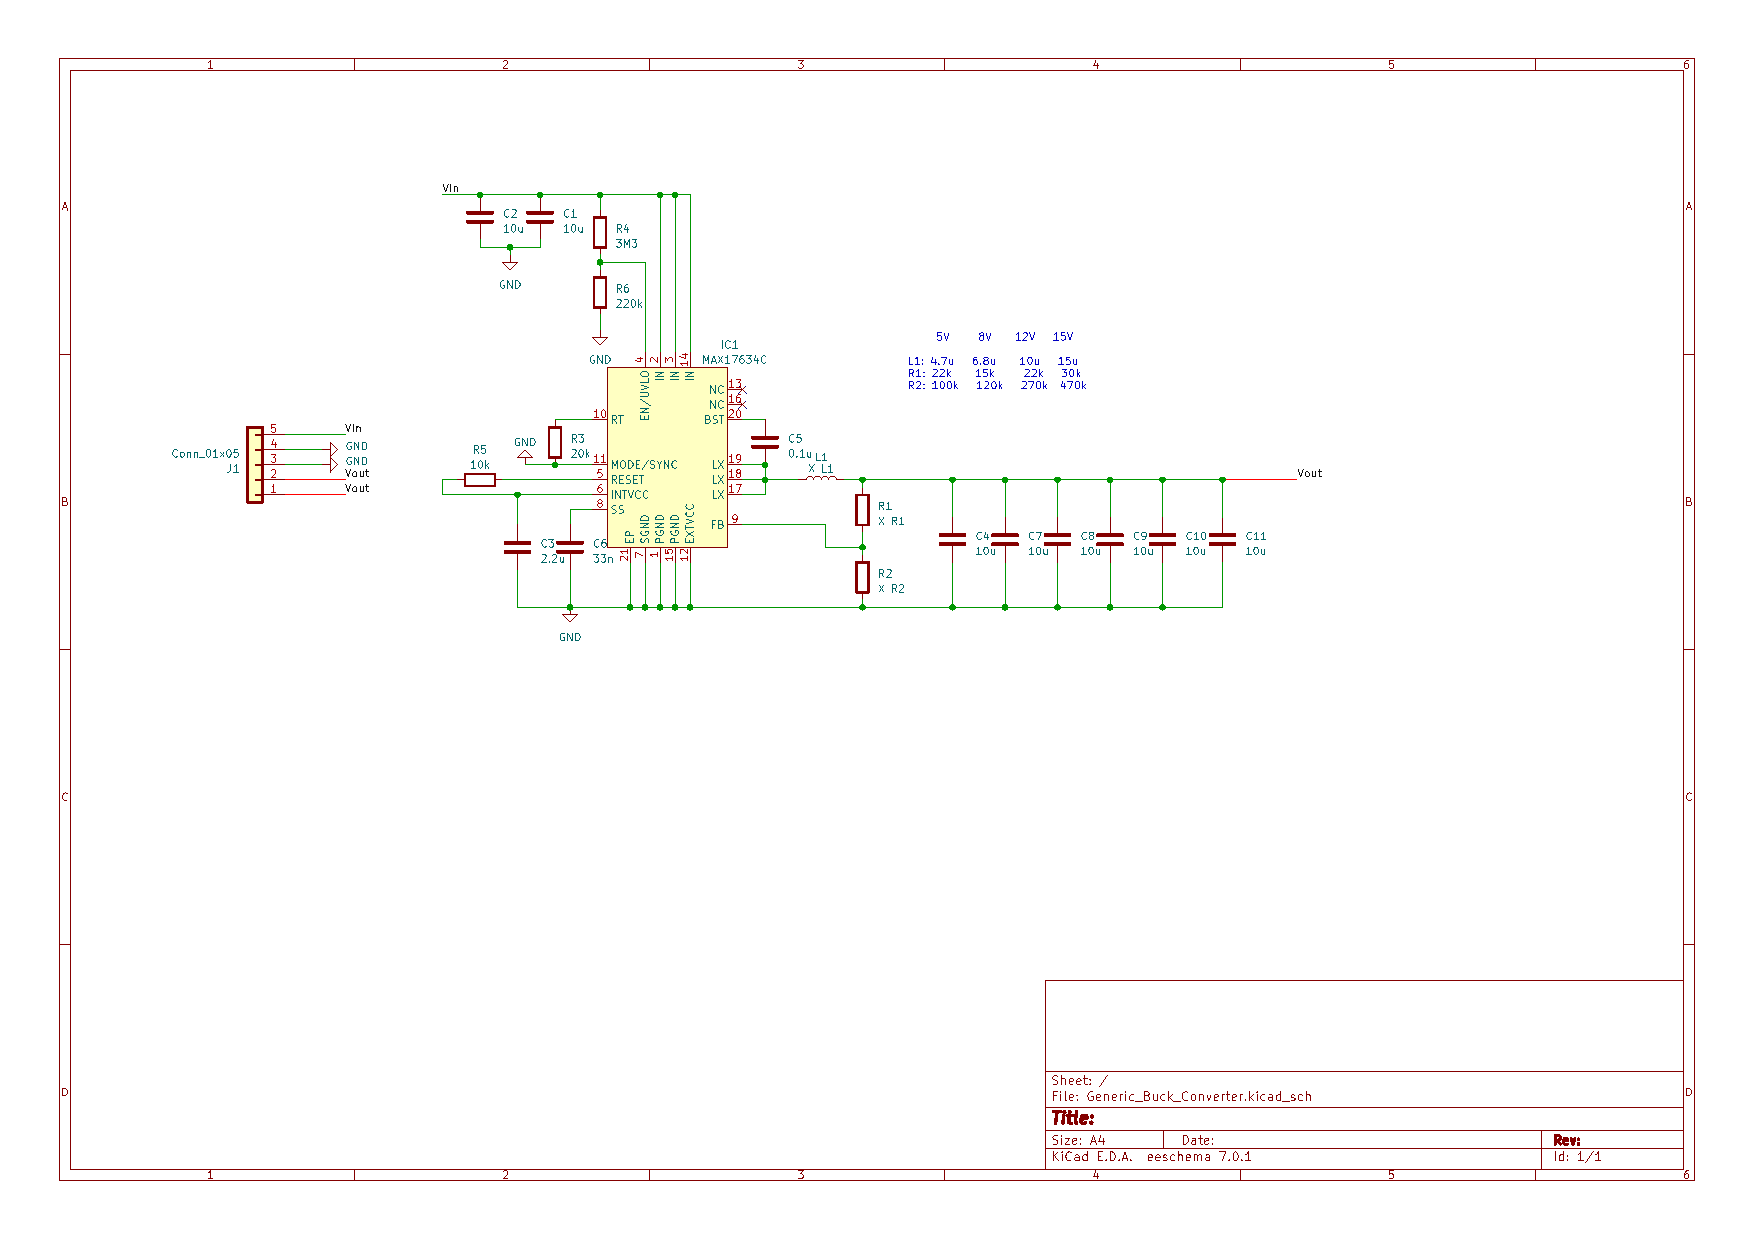
\includegraphics[angle=90, width=\linewidth, height=0.9\textheight, keepaspectratio]{Generic_Buck_Converter_schematic.pdf}
    \caption{Schematic of Buck Converter}
    \label{fig:buck-schematic}
\end{figure}

\section*{SEPIC schematic} \label{Appendix_SEPIC_schematic}
\addcontentsline{toc}{section}{SEPIC schematic}  
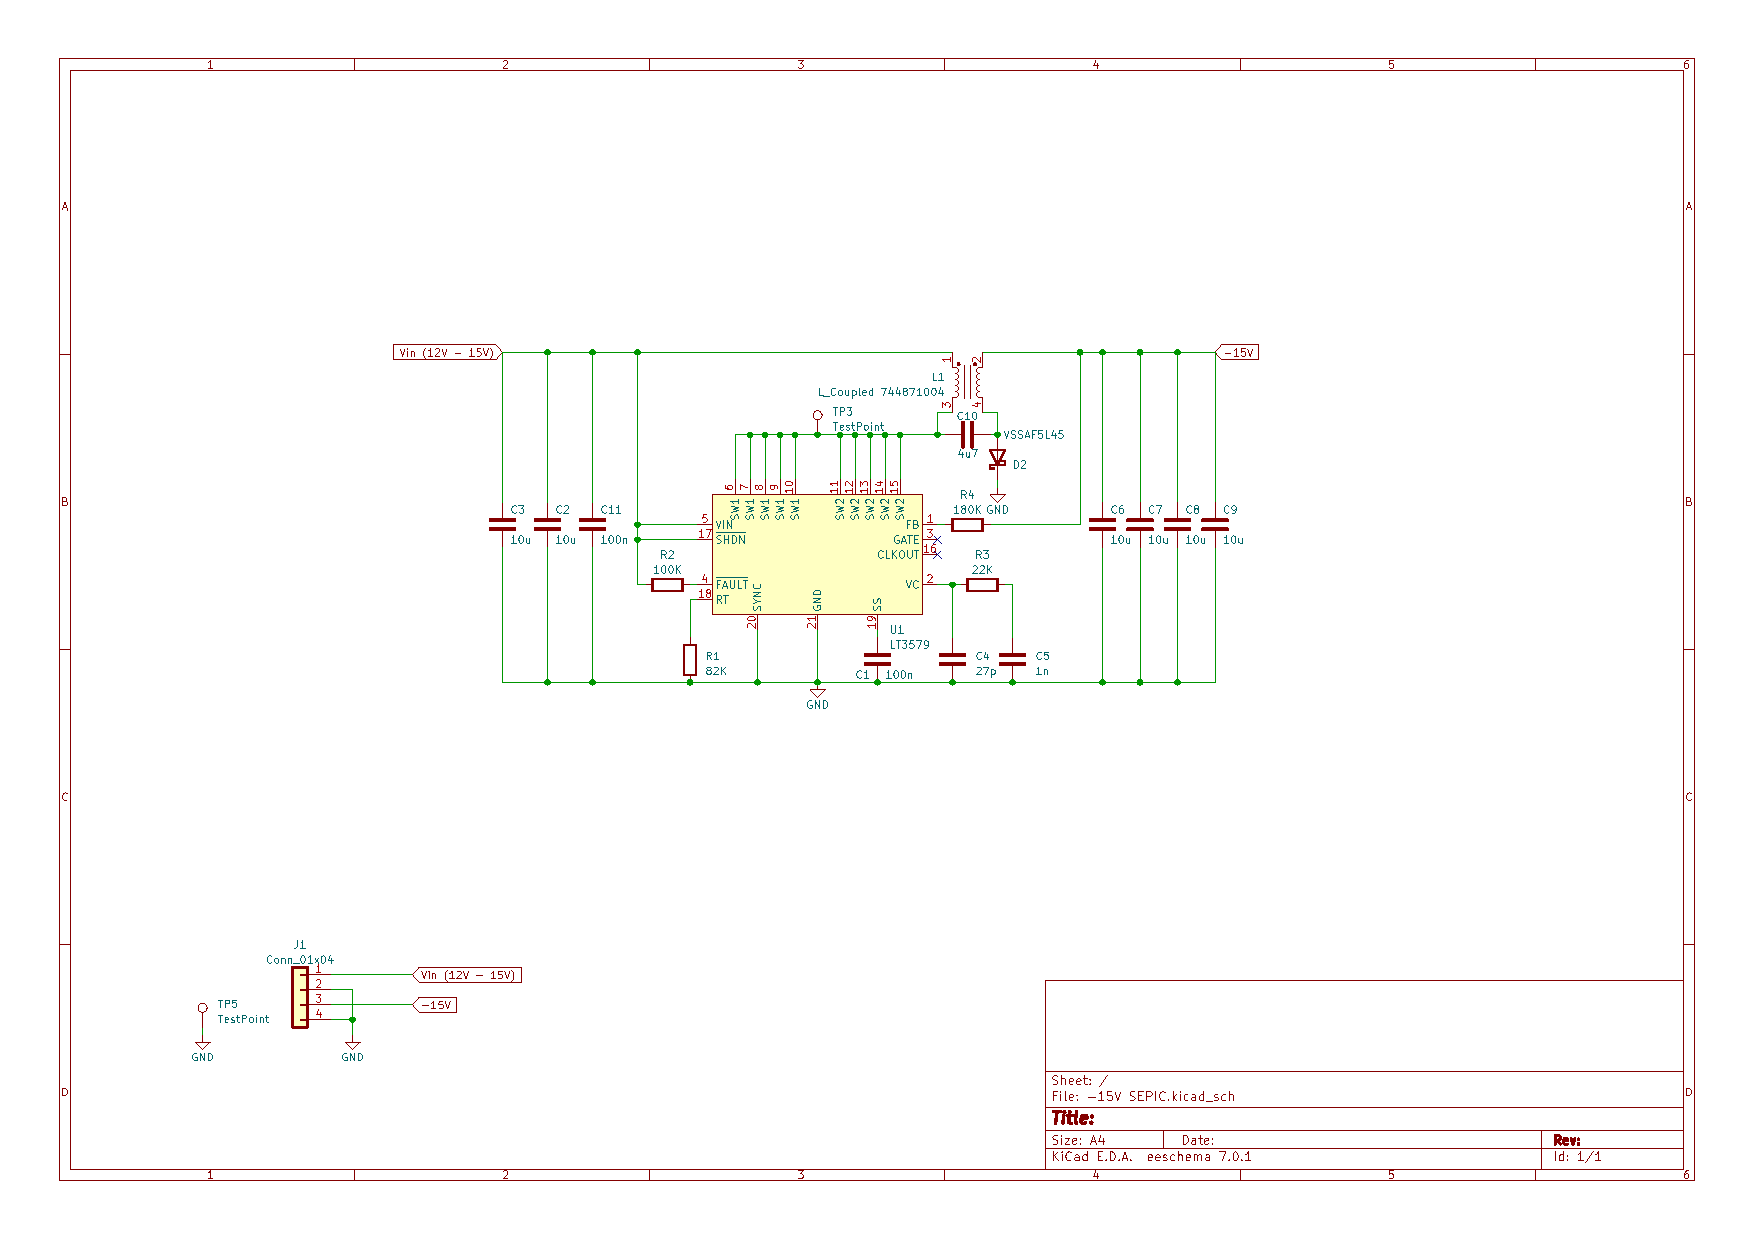
\includegraphics[angle=90, width=500pt]{-15V_SEPIC_schematic.pdf}

\section*{Linear regulator schematic}\label{Appendix_lin_schematic}
\addcontentsline{toc}{section}{Linear regulator schematic}  
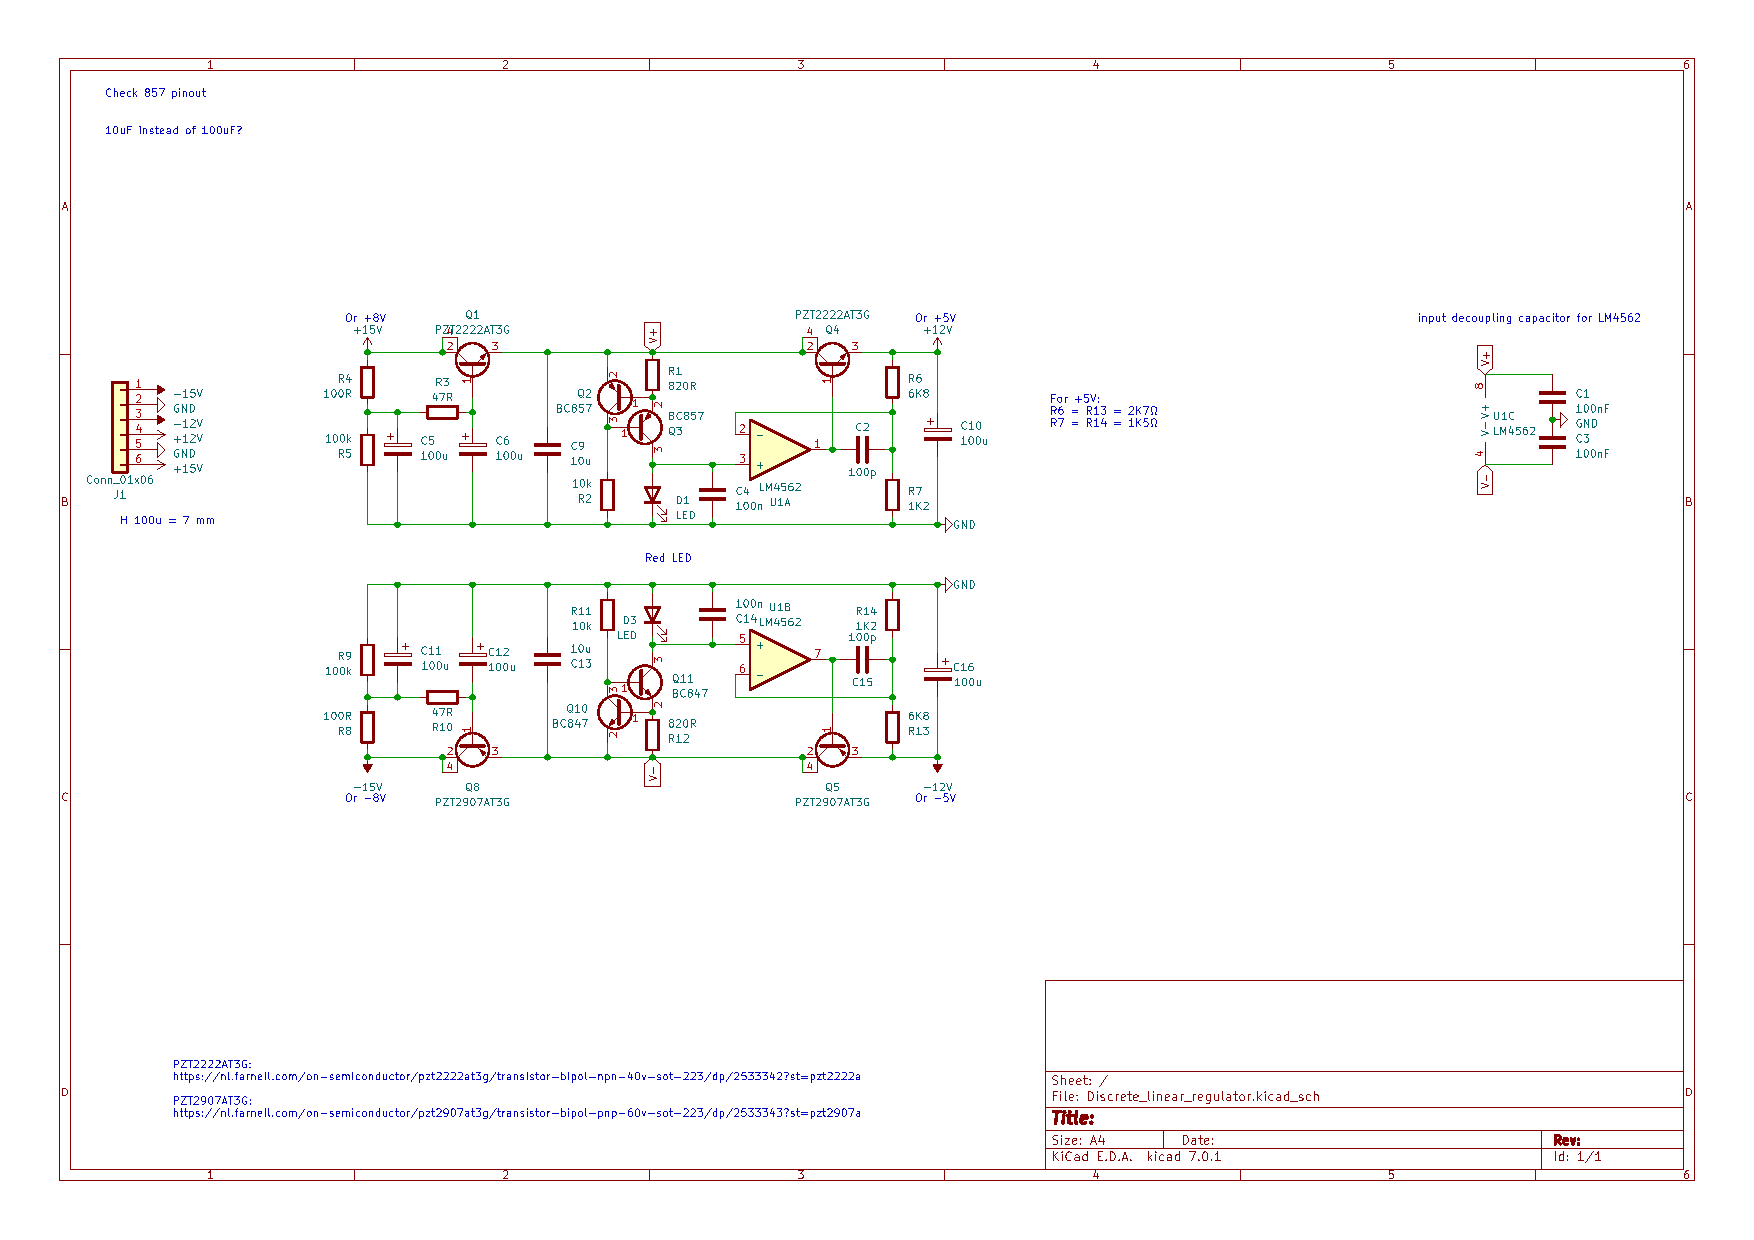
\includegraphics[angle=90, width=500pt]{Discrete_linear_regulator_schematic.pdf}

\section*{Main board schematic} \label{Appendix_main_schematic}
\addcontentsline{toc}{section}{Main board schematic}  
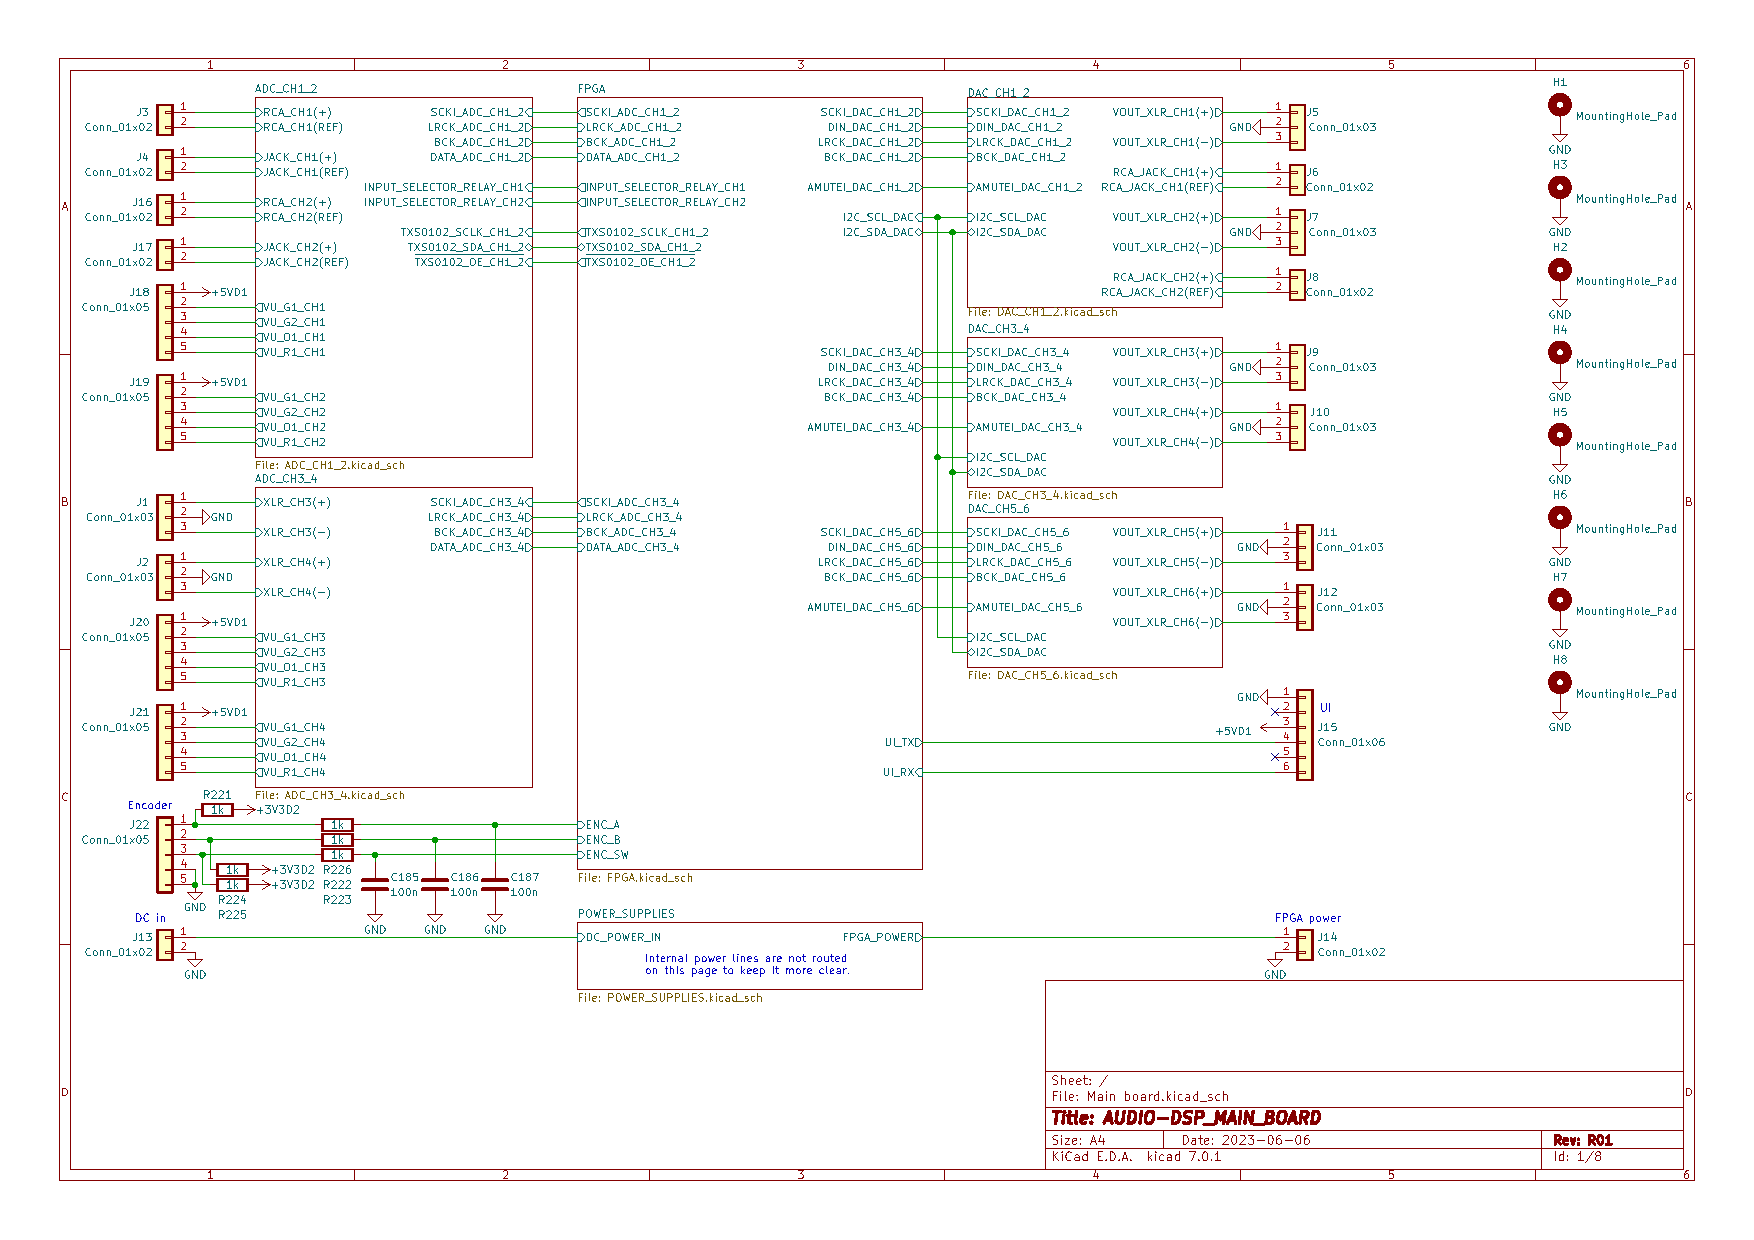
\includepdf[angle=90, pages=-]{Main_board_schematic.pdf}

\section*{Buck converter calculations} \label{Appendix_buck_calculations}
\addcontentsline{toc}{section}{Buck converter calculations}  
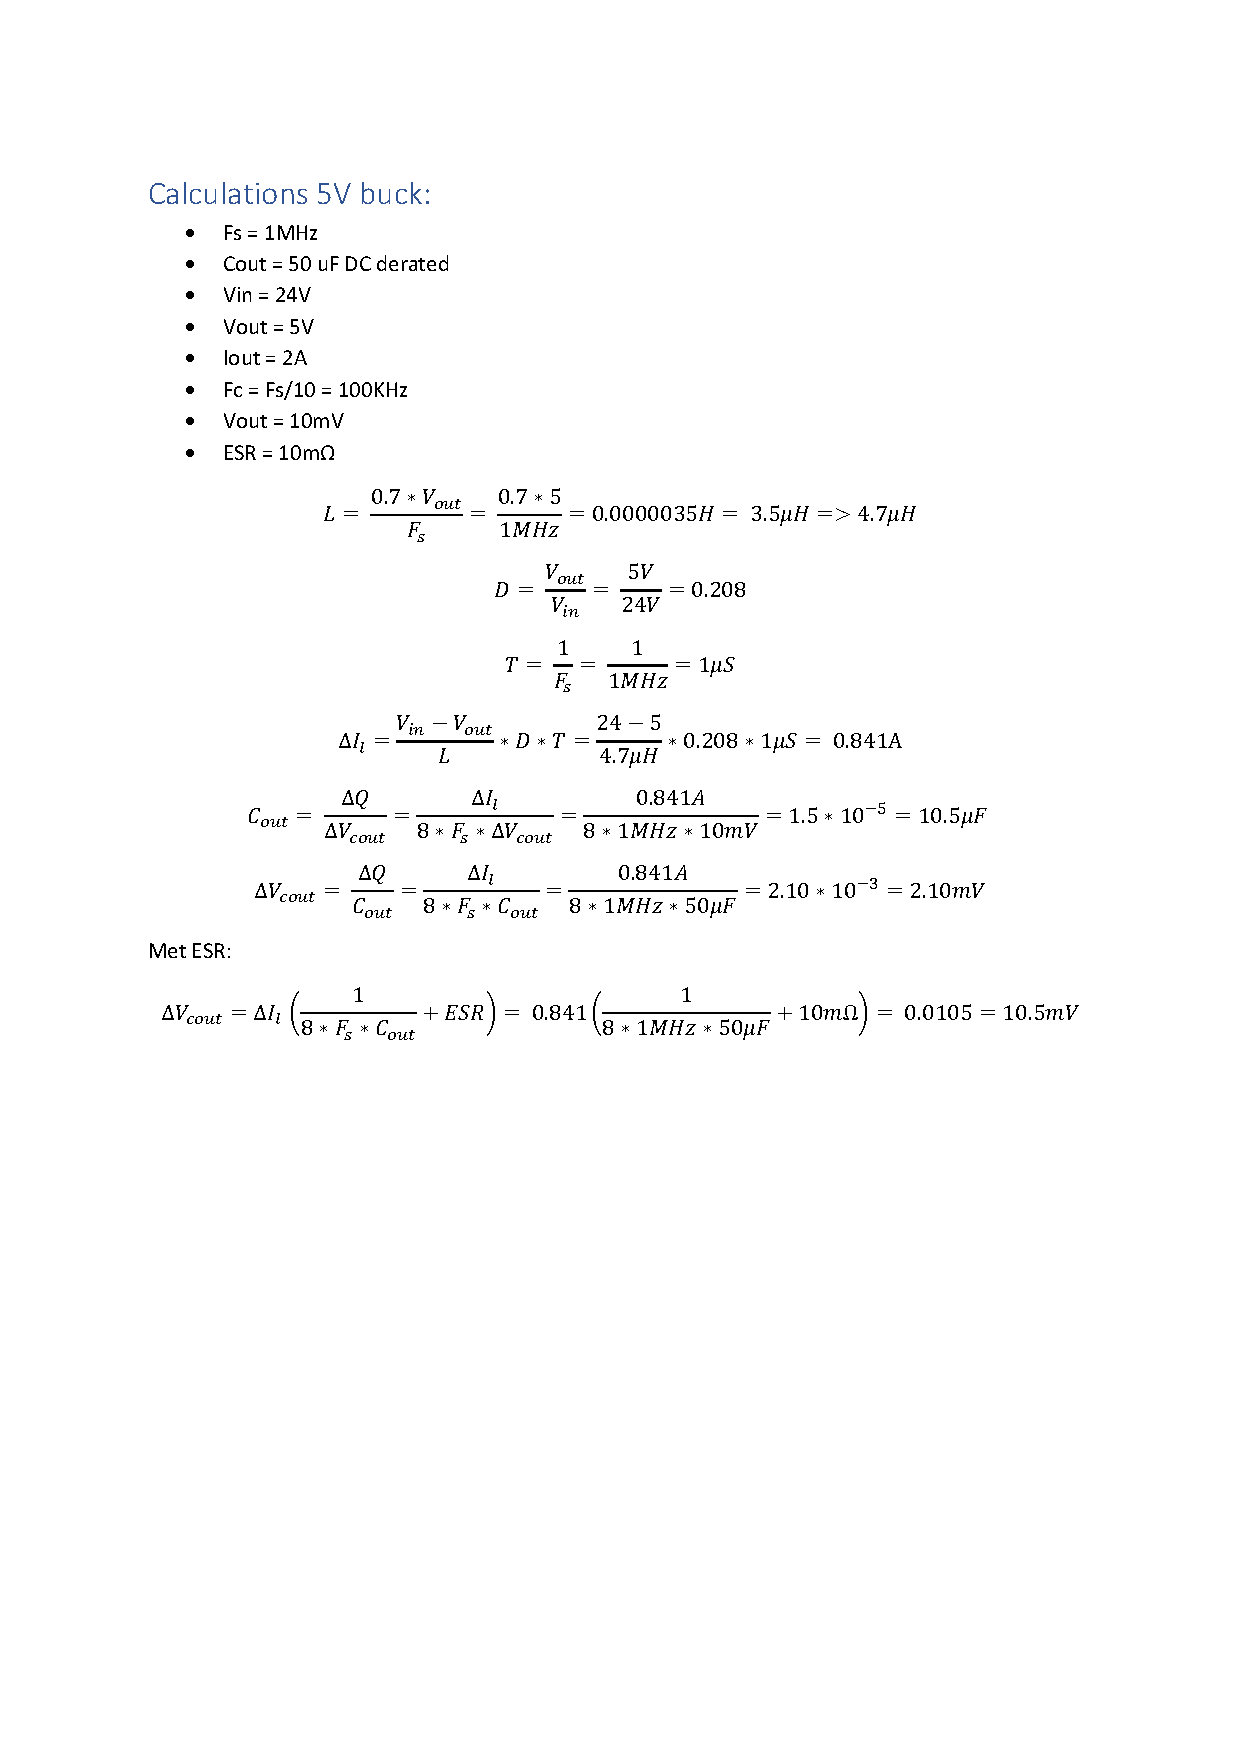
\includepdf[pages=-]{Calculations_buck_converter.pdf}

\section*{SEPIC calculations} \label{Appendix_SEPIC_calculations}
\addcontentsline{toc}{section}{SEPIC calculations}  
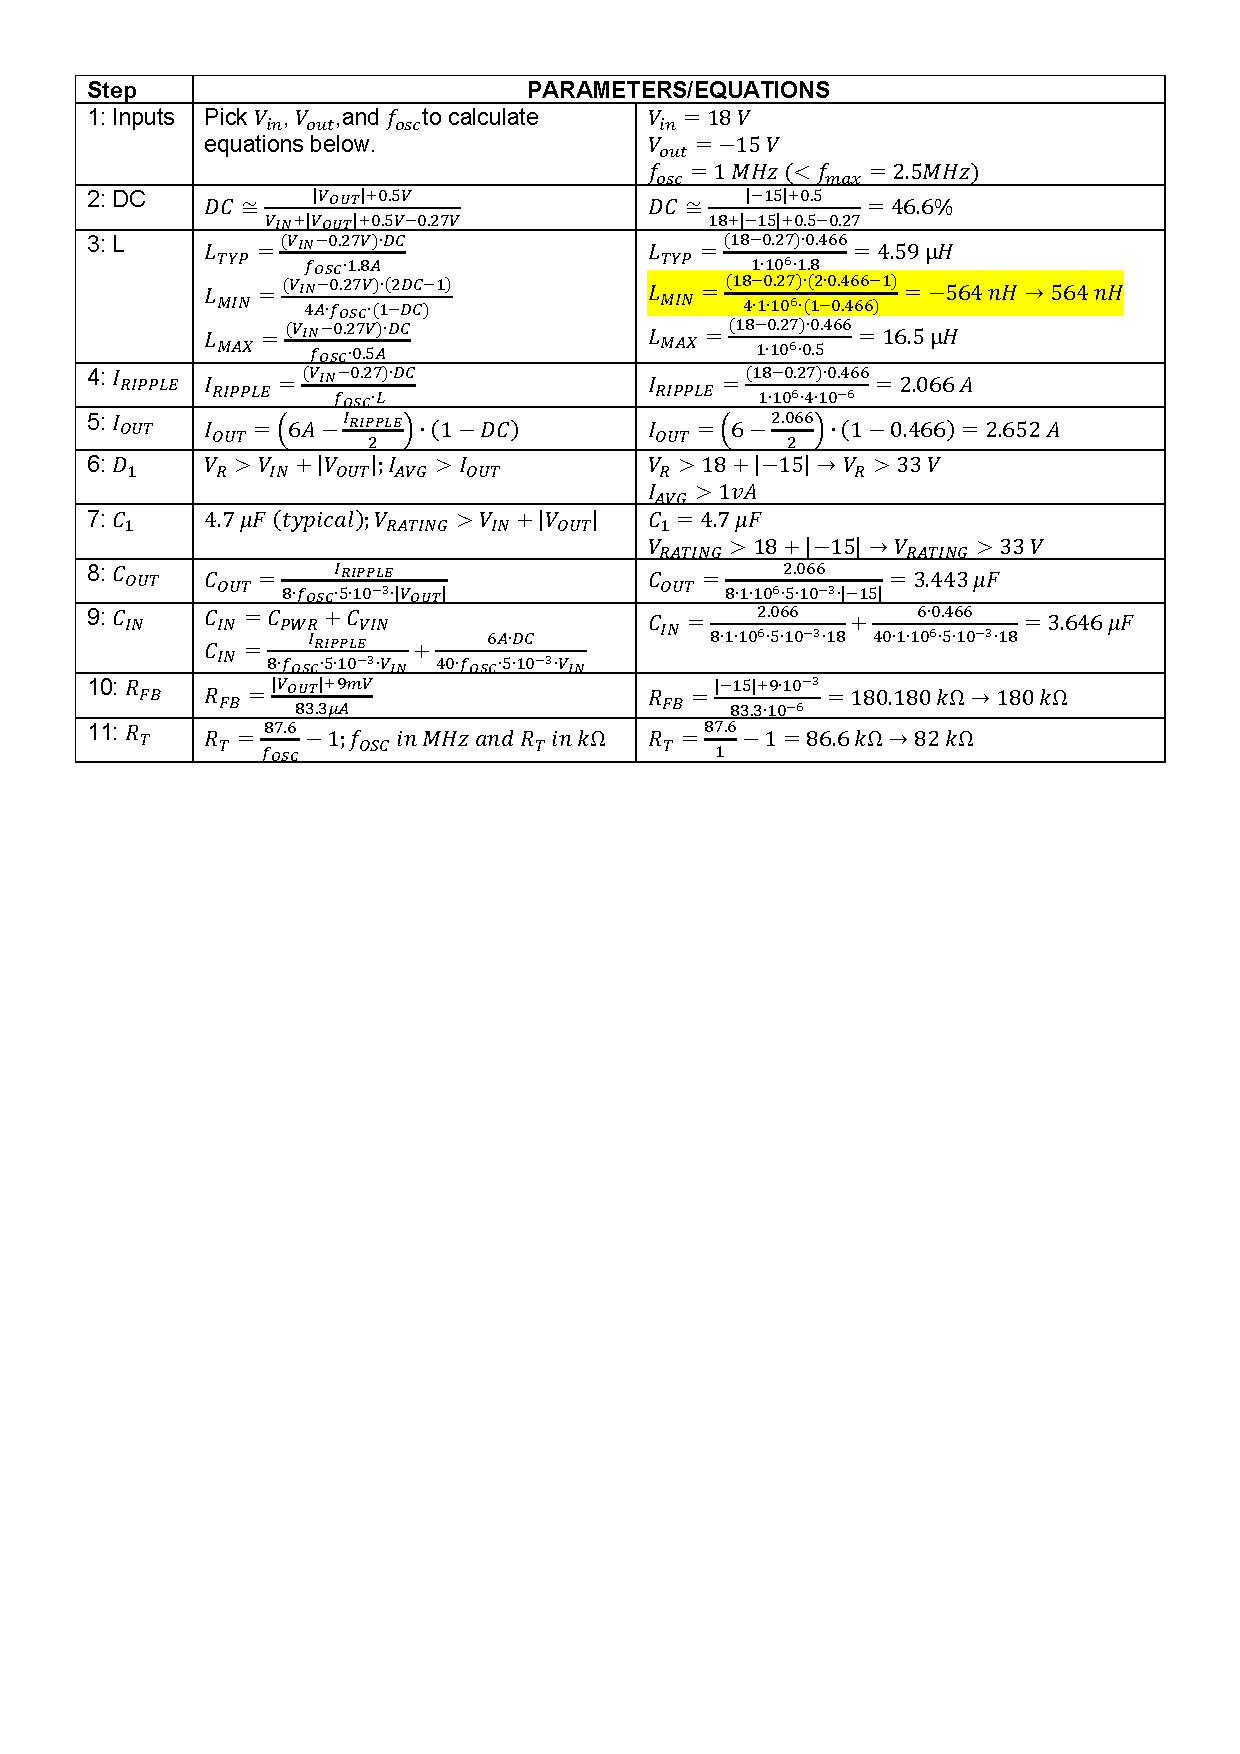
\includepdf[pages=-]{LT3579_calculations.pdf}
